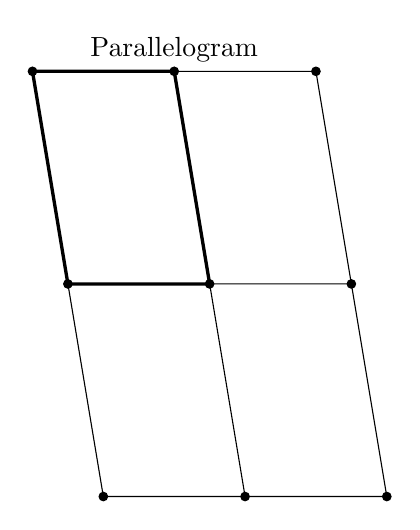
\begin{tikzpicture}[scale=1.8]

%draw the parallelogram lattice
\coordinate (parallelogram) at (-2.5,3);
\node [above] at (parallelogram) {Parallelogram};

\draw (-1,0) -- (-3,0) -- (-3.5,3) -- (-1.5,3) -- cycle;
\draw  (-2,0) -- (-2.5,3)  (-3.25,1.5) -- (-1.25,1.5);
\draw [very thick] (-3.25,1.5) -- (-3.5,3) -- (-2.5,3) -- (-2.25,1.5) -- cycle;
\foreach \x in {-1,-2,-3} \filldraw[fill=black, draw=black] (\x,0) circle (0.03);
\foreach \x in {-1.25,-2.25,-3.25} \filldraw[fill=black, draw=black] (\x,1.5) circle (0.03);
\foreach \x in {-1.5,-2.5,-3.5} \filldraw[fill=black, draw=black] (\x,3) circle (0.03);


\end{tikzpicture}

